\documentclass[
10pt, % Set the default font size, options include: 8pt, 9pt, 10pt, 11pt, 12pt, 14pt, 17pt, 20pt
%t, % Uncomment to vertically align all slide content to the top of the slide, rather than the default centered
aspectratio=169, % Uncomment to set the aspect ratio to a 16:9 ratio which matches the aspect ratio of 1080p and 4K screens and projectors
]{beamer}

\usepackage[all]{xy}

\usepackage[spanish]{babel}
\usepackage[utf8]{inputenc}

\graphicspath{{Images/}{./}} % Specifies where to look for included images (trailing slash required)

\usepackage{booktabs} % Allows the use of \toprule, \midrule and \bottomrule for better rules in tables

%\usepackage{tikz}
%\usetikzlibrary{positioning}
%\usetikzlibrary{shapes,arrows,arrows,positioning,fit}

\usepackage{tikz}
\usetikzlibrary{mindmap}
\usetikzlibrary{arrows, positioning}
\usetikzlibrary{arrows, shapes, positioning, shadows, trees}

\usepackage{forest}

\usepackage{multirow}

\usepackage{graphicx}
\usepackage{hyperref}

\usepackage{xcolor,listings}
\usepackage{textcomp}
%\usepackage{color}

\usepackage{enumitem}

\usepackage{xcolor}

\usepackage{verbatim}
\usepackage{changepage}

\usepackage{algpseudocode}
\usepackage{gensymb}

\usepackage{venndiagram}

\usepackage{graphicx}
% \usepackage{media9}

% \usepackage{algorithm}
% \usepackage{algorithmic}

\providecommand{\abs}[1]{\lvert#1\rvert}

%----------------------------------------------------------------------------------------
%	SELECT LAYOUT THEME
%----------------------------------------------------------------------------------------
\usetheme{Madrid} 

%----------------------------------------------------------------------------------------
%	SELECT COLOR THEME
%----------------------------------------------------------------------------------------
%\usecolortheme{beaver}
%\usecolortheme{seahorse}
\usecolortheme{spruce} % verde suave
%\usecolortheme{whale}
%\usecolortheme{wolverine}

%----------------------------------------------------------------------------------------
%	SELECT FONT THEME & FONTS
%----------------------------------------------------------------------------------------
\usefonttheme{default} % Typeset using the default sans serif font
%\usefonttheme{serif} % Typeset using the default serif font (make sure a sans font isn't being set as the default font if you use this option!)
%\usefonttheme{structurebold} % Typeset important structure text (titles, headlines, footlines, sidebar, etc) in bold
%\usefonttheme{structureitalicserif} % Typeset important structure text (titles, headlines, footlines, sidebar, etc) in italic serif
%\usefonttheme{structuresmallcapsserif} % Typeset important structure text (titles, headlines, footlines, sidebar, etc) in small caps serif

%------------------------------------------------

%\usepackage{mathptmx} % Use the Times font for serif text
%\usepackage{palatino} % Use the Palatino font for serif text

\usepackage{helvet} % Use the Helvetica font for sans serif text
%\usepackage[default]{opensans} % Use the Open Sans font for sans serif text
%\usepackage[default]{FiraSans} % Use the Fira Sans font for sans serif text
\usepackage[default]{lato} % Use the Lato font for sans serif text

%----------------------------------------------------------------------------------------
%	SELECT INNER THEME
%----------------------------------------------------------------------------------------
\useinnertheme{circles}


\setbeamertemplate{footline} % Uncomment this line to remove the footer line in all slides
%\setbeamertemplate{footline}[page number] % Uncomment this line to replace the footer line in all slides with a simple slide count

\setbeamertemplate{navigation symbols}{} % Uncomment this line to remove the navigation symbols from the bottom of all slides

%----------------------------------------------------------------------------------------
%	PRESENTATION INFORMATION
%----------------------------------------------------------------------------------------

\title[Short Title]{Representación del conocimiento \\ Indexación y Almacenamiento} 

\subtitle{Sistemas de Recuperación de Información}

\author{Lic. Carlos León González \\ Dra.C. Lucina García Hernández}

\institute[UC]{Facultad de Matem\'atica y Computaci\'on \\ Universidad de La Habana \\ \smallskip }

\date{26 de febrero de  2024} % Presentation date or conference/meeting name, the optional parameter can contain a shortened version to appear on the bottom of every slide, while the required parameter value is output to the title slide

%----------------------------------------------------------------------------------------

\begin{document}
	
	\lstset{
		literate=%
		{á}{{\'a}}1
		{í}{{\'i}}1
		{é}{{\'e}}1
		{ý}{{\'y}}1
		{ú}{{\'u}}1
		{ó}{{\'o}}1
		{ě}{{\v{e}}}1
		{š}{{\v{s}}}1
		{č}{{\v{c}}}1
		{ř}{{\v{r}}}1
		{ž}{{\v{z}}}1
		{ď}{{\v{d}}}1
		{ť}{{\v{t}}}1
		{ň}{{\v{n}}}1                
		{ů}{{\r{u}}}1
		{Á}{{\'A}}1
		{Í}{{\'I}}1
		{É}{{\'E}}1
		{Ý}{{\'Y}}1
		{Ú}{{\'U}}1
		{Ó}{{\'O}}1
		{Ě}{{\v{E}}}1
		{Š}{{\v{S}}}1
		{Č}{{\v{C}}}1
		{Ř}{{\v{R}}}1
		{Ž}{{\v{Z}}}1
		{Ď}{{\v{D}}}1
		{Ť}{{\v{T}}}1
		{Ň}{{\v{N}}}1                
		{Ů}{{\r{U}}}1    
	}
	
	
	\begin{frame}
		\titlepage
	\end{frame}
	
	%------------------------------------------------
	% Objetivos
	\begin{frame}
		
		\frametitle{Objetivos}
		
		\begin{itemize}

			\item Comprender el concepto de conocimiento y razonamiento en el ámbito de la computación
			
			\item Presentar diversas formas de representaciones del conocimiento
			
			\item Definir y comprender diferentes tipos de indexación
						
		\end{itemize}
		
	\end{frame}
	
	%------------------------------------------------
	% Necesidad para la IA
	\begin{frame}
		
		\frametitle{¿Conocimiento?}
		
		La representación del conocimiento y el razonamiento están en el centro del gran desafío de la Inteligencia Artificial: comprender la naturaleza de la inteligencia y la cognición tan bien que se pueda hacer que las computadoras exhiban habilidades similares a las humanas.
		
		\pause
		\vspace{2\baselineskip}
		\textcolor{purple}{¿Pero qué es el conocimiento en computación?}
		
		% La cognición es la facultad de un ser vivo para procesar información a partir de la percepción, el conocimiento adquirido y características subjetivas que permiten valorar la información.
		
		\pause
		\begin{alertblock}{}
			Representación de símbolos formales para representar una colección de proposiciones válidas.
		\end{alertblock}
		
	\end{frame}
	
	
	%------------------------------------------------
	% Necesidad del conocimiento
	\begin{frame}
		
		\frametitle{Necesidad de tener conocimiento en los sistemas}
		
		Para sistemas suficientemente complejos, a veces es útil describir los sistemas en términos de \textbf{creencias}, \textbf{objetivos}, \textbf{miedos} e \textbf{intenciones}.
		
		\vspace{2\baselineskip}
		Ejemplo: \\
			\hspace{2mm} ``Porque creía que su reina estaba en peligro, pero aún quería controlar el centro del tablero.''
			
		\vspace{1\baselineskip}
		\hspace{2mm} Justificación del porqué una máquina efectúo una determinada jugada en el ajedrez.
		
	\end{frame}
	
	%------------------------------------------------
	% Uso final del conocimiento
	\begin{frame}
		
		\frametitle{Uso final del conocimiento}
		
		Un objetivo de tener bases de conocimiento en los sistemas es que los programas cuenten con la capacidad de ``razonar'' lo cual le permita tomar decisiones.
		
		\pause
		\vspace{2\baselineskip}
		\textcolor{purple}{¿Pero qué es el razonamiento en computación?}
				
		\pause
		\begin{alertblock}{}
			Es la manipulación formal de los símbolos que representan una colección de proposiciones válidas y conocidas para producir representaciones de nuevas proposiciones. 
		\end{alertblock}
		
		\pause
		\vspace{2\baselineskip}
		Luego, tener una correcta representación del conocimiento permite arribar a resultados precisos en posteriores etapas.
		
	\end{frame}
	
	%------------------------------------------------
	% 
	\begin{frame}
		
		\frametitle{Estructura del conocimiento}
		
		\begin{centering }
			
		\begin{tikzpicture}
			
			% Dibujar el triángulo por parte
			\draw (2, 0) -- (3,1.4) -- (7,1.4) -- (8,0) -- cycle;
			\draw (3,2.1) -- (4,3.5) -- (6,3.5) -- (7,2.1) -- cycle;
			\draw (4,4.2) -- (5,6) -- (6,4.2) -- cycle;
		
			% Colorear
			\fill[cyan!10!] (2, 0) -- (3,1.4) -- (7,1.4) -- (8,0) -- cycle;
			\fill[cyan!40!] (3,2.1) -- (4,3.5) -- (6,3.5) -- (7,2.1) -- cycle;
			\fill[cyan!90!] (4,4.2) -- (5,6) -- (6,4.2) -- cycle;
			
			% Dibujar nodos
			\node (A) at (2.5,0.8) {};
			\node (B) at (3.5,2.84) {};
			\node (C) at (4.5,5) {};
			
			% Dibujar las flechas
			\draw[->, thick] (5,1.14) -- (5,2.4);
			\draw[->, thick] (5,3.16) -- (5,4.54);
			
			% Etiquetas de las capas
			% Pirámide
			\node at (5,0.6) {\textbf{Dato}};
			\node at (5,2.8) {\textbf{Información}};
			\node at (5,5) {\textbf{Conocimiento}};
			% Transición
			\node at (6,1.75) {+ Contexto};
			\node at (6.1,3.8) {+ Significado};
			% Datos
			\node[align=left] at (9.3,0.7) {Tigre\\Carnívoro};
			\node[align=left] at (10.8,2.8) {El tigre puede medir hasta 3.1 metros de largo.\\El tigre es carnívoro.};
			\node[align=left] at (9.3,5) {El tigre es un felino peligroso.\\No existe un felino mayor al tigre.};
			
		\end{tikzpicture}
		
		\end{centering }
	
	\end{frame}
	
	%------------------------------------------------
	% 
	\begin{frame}
		
		\frametitle{Tipos de conocimiento}
		
		\begin{itemize}
			\item \textcolor<3-6>{gray}{Conocimiento declarativo}
			\only<2>{
				\begin{itemize} 
					\item Se refiere al ``qué''
					\item Abarca idea, hechos y objetos
					\item Describe el conocimiento
				\end{itemize}
			}
						
			\item \textcolor<2, 4-6>{gray}{Conocimiento estructural}
			\only<3>{
				\begin{itemize}
					\item Se refiere al ``cómo se relacionan las cosas''
					\item Establece relaciones entre varios conceptos como: naturaleza, componente o agrupación
					\item Necesario para la resolución de problemas
				\end{itemize}
			}
			
			\item \textcolor<2-3, 5-6>{gray}{Conocimiento procesal}
			\only<4>{
				\begin{itemize}
					\item Se refiere al conocimiento práctico y depende de la tarea
					\item Abarca políticas, estrategias y conocimientos responsables de la toma de decisión
					\item Es un conocimiento imperativo
				\end{itemize}
			}
			
			\item \textcolor<2-4, 6>{gray}{Metaconocimiento}
			\only<5>{
				\begin{itemize}
					\item Se refiere a ``lo que ya se conoce''
					\item Es conocimiento sobre el conocimiento, entiéndase como categorías, planes y aprendizajes pasados
				\end{itemize}
			}
			
			\item \textcolor<2-5>{gray}{Conocimiento heurístico}
			\only<6>{
				\begin{itemize}
					\item Se refiere a ``aprender de la experiencia''
					\item Ayuda a la máquina a tomar decisiones futuras basadas en experiencias pasadas 
					\item Brinda enfoques alternativos que quizás funcione pero que no se garantiza su efectividad
				\end{itemize}
			}
			
		\end{itemize}
		
		\only<7->{
			\vspace{2\baselineskip}
			\begin{centering}
				
				\textbf{\large{La representación del conocimiento es de suma importancia para los sistemas e influye en el razonamiento}}
					
			\end{centering}
		}
		
		\only<8>{
			\vspace{2\baselineskip}
			\textcolor{purple}{¿Cómo se representa el conocimiento?}
		}
		
	\end{frame}
	
	%------------------------------------------------
	% Modelos de representación del conocimiento
	\begin{frame}
		
		\frametitle{Algunos modelos de representación del conocimiento}
		
		\begin{enumerate}
			\item Basado en reglas
			\item Orientado a objetos (marcos)
			\item Basado en herencia (redes semánticas)
		\end{enumerate}
		
		% La representación del conocimiento es una forma natural de ver al mundo.
		% La obstracción influye en el razonamiento.
		
	\end{frame}
	
	%------------------------------------------------
	% Modelo de representación del conocimiento basado en reglas
	\begin{frame}
		
		\frametitle{Modelo de representación del conocimiento basado en reglas}
		
		\begin{itemize}
			
			\item La información está dispersa en axiomas y contextos.

			\vspace{1\baselineskip}
			\item Se define sobre la condición o regla \texttt{IF - THEN} en su forma
			$$\texttt{IF}\ condiciones\ \ \texttt{THEN}\ acciones$$
			
			\vspace{1\baselineskip}			
			\item Una condición $P \Rightarrow Q$ puede entenderse como una transformación de 
			\begin{itemize}
				\item las afirmaciones de $P$ a las afirmaciones de $Q$, o
				\item las metas de $Q$ a las metas de $P$.
			\end{itemize}
			
			\vspace{1\baselineskip}
			\item El razonamiento es activado en cadena hacia delante cuando se consumen las reglas de producción.
			
			\vspace{1\baselineskip}
			\item El lenguaje \textbf{Prolog} es la materialización de esta representación.
					
		\end{itemize}
		
	\end{frame}
	
	%------------------------------------------------
	% Ejemplo del conocimiento por reglas
	\begin{frame}
		
		\frametitle{Ejemplo del conocimiento por reglas}
				
		\begin{block}{Ejemplo}
			\texttt{IF} x $=$ pájaro \texttt{THEN} puede\_volar \\
			\texttt{IF} x $=$ pájaro $\land$ peso $>$ 100 \texttt{THEN} no\_puede\_volar \\
			\texttt{IF} x $=$ pájaro $\land$ x = pinguino \texttt{THEN} no\_puede\_volar \\
			\texttt{IF} x $=$ no\_pájaro \texttt{THEN} no\_puede\_volar 
		\end{block}
		
		\vspace{2\baselineskip}
		
		\only<1>{
			\begin{itemize}
				\item Se muestra un conjunto reglas para definir cuando un animal vuela.
				
				\vspace{1\baselineskip}
				
				\item Se pueden efectuar dos tipos de razonamiento:
				\begin{itemize}
					\item basado en los datos y,
					\item basado en las ganancias.
				\end{itemize}
				
			\end{itemize}
		}
		
		\only<2>{
			Usando las reglas definidas ...
			\begin{enumerate}
				\item \textcolor{purple}{¿El águila puede volar?}
				\item \textcolor{purple}{¿El pingüino puede volar?}
				\item \textcolor{purple}{¿El avestruz puede volar?}
			\end{enumerate}		
		}
		
	\end{frame}
	
	%------------------------------------------------
	% Resolución de conflictos en los sistemas basados en reglas
	\begin{frame}
		
		\frametitle{Resolución de conflictos en los sistemas basados en reglas}
		
		\begin{itemize}
			\item El orden de presentación de las reglas importa.
			
			\vspace{1\baselineskip}
			\item Mientras mayor sea el nivel de especificidad en la reglas mayor será la exactitud del razonamiento, pero aumenta con ello el espacio en la memoria.
			
			\vspace{1\baselineskip}
			\item Existen políticas para la consultas de las reglas y los llamados recursivos que pudiesen existir entre ellas.
			
		\end{itemize}
	
	\end{frame}
	
	%------------------------------------------------
	% Modelo de representación del conocimiento orientado a objetos
	\begin{frame}
		
		\frametitle{Modelo de representación del conocimiento orientado a objetos}
		
		\begin{itemize}
			
			\only<1>{
			
				\item Ordenar la información depende de la capacidad de ver y representar el mundo como objeto. \\Por ejemplo: 
				\begin{itemize}
					\item Objeto físico: mesa.
					\item Características del objeto físico: color, tamaño, material, etc.
					\item Objeto no físico: viaje.
					\item Características del objeto no físico: destino, lugar de partida, personas, tiempo de demora, etc.
				\end{itemize}
				
				\vspace{1\baselineskip}
				\item Usa funciones de agrupación para establecer relaciones entre los objetos y sus partes descriptivas.
				
			}
			
			\only<2>{
				
				\item El tipo de razonamiento se basa en tres ideas fundamentales:
				\begin{enumerate}
					\item Reconocer la situación y activar las representaciones de objetos relevantes.
					\item Usar los objetos activados para establecer expectativas.
					\item Desarrollar la situación una vez reconocida.
				\end{enumerate}
				
				\vspace{1\baselineskip}
				\item Utilizado en reconocimiento de relaciones, como por ejemplo en la comprensión de historias, en el monitoreo de datos y en la propagación y la aplicación de restricciones para tareas de planificación.
			
			}
			
		\end{itemize}
		
	\end{frame}
	
	%------------------------------------------------
	% Estructura del conocimiento orientado a objetos
	\begin{frame}
		
		\frametitle{Estructura del conocimiento orientado a objetos}
		
		\begin{itemize}
			\item El conocimiento se define en estructuras conocidas como \textbf{marco}.
			
			\vspace{1\baselineskip}
			\item Existen dos tipos de marco:
			\begin{itemize}
				
				\begin{minipage}[t]{0.43\textwidth} % Primera columna
					
					\item Individual: se refiere a objetos simples, como una persona.
					
					\vspace{.5\baselineskip}
					Representación: \\
					\texttt{(nombre\_marco\\   
						      nombre\_ranura\_1 valor\_atómico\_1\\
						\hspace{2cm} nombre\_ranura\_2 valor\_atómico\_2\\
						...)}
					
				\end{minipage}
				\hfill  % Espacio entre las columnas
				\begin{minipage}[t]{0.43\textwidth} % Segunda columna
					
					\item Genérico: se refiere a categorías de objetos, como estudiante.
					
					\vspace{.5\baselineskip}
					Misma representación pero los valores pueden ser más complejos, como un procedimiento.
					
				\end{minipage}
				
			\end{itemize}
							
			\vspace{1\baselineskip}
			\item Permite definir particularizaciones e instancias  de objetos generales.
			
			\vspace{1\baselineskip}
			\item Simula la programación orientada a objetos.
			
		\end{itemize}
		
	\end{frame}
	
	%------------------------------------------------
	% Razonamiento usando marcos
	\begin{frame}
		
		\frametitle{Razonamiento usando marcos}
		
		% Tipos de razonamiento. Cada uno se define sobre lo que se activa o utiliza. 
		
		\begin{itemize}
			\item Local o básico
			\begin{itemize}
				\item Uso de las instancias de los marcos 
				\item Uso de los procedimientos aplicados a los marcos
			\end{itemize}
			
			\vspace{1\baselineskip}
			\item Global
			\begin{itemize}
				\item Creación de marcos generales 
				\item Uso de restricciones con las ranuras
			\end{itemize}
			
		\end{itemize}
		
	\end{frame}
	
	%------------------------------------------------
	% Ejemplo de la representación usando marcos
	\begin{frame}
		
		\frametitle{Ejemplo de la representación usando marcos}
		
		\begin{minipage}{.3\textwidth}
			
			La representación es un ejemplo de un viaje con estancia.
			
			\vspace{2\baselineskip}
			Usando la representación anterior, ¿cómo puedo ...
			\begin{enumerate}
				\item \textcolor{purple}{conocer la cantidad de días que tomará el viaje?}
				\item \textcolor{purple}{saber el costo total del viaje?}
			\end{enumerate}		
			
		\end{minipage}%
		\hfill
		\begin{minipage}{.6\textwidth}
			
			\centering
			
			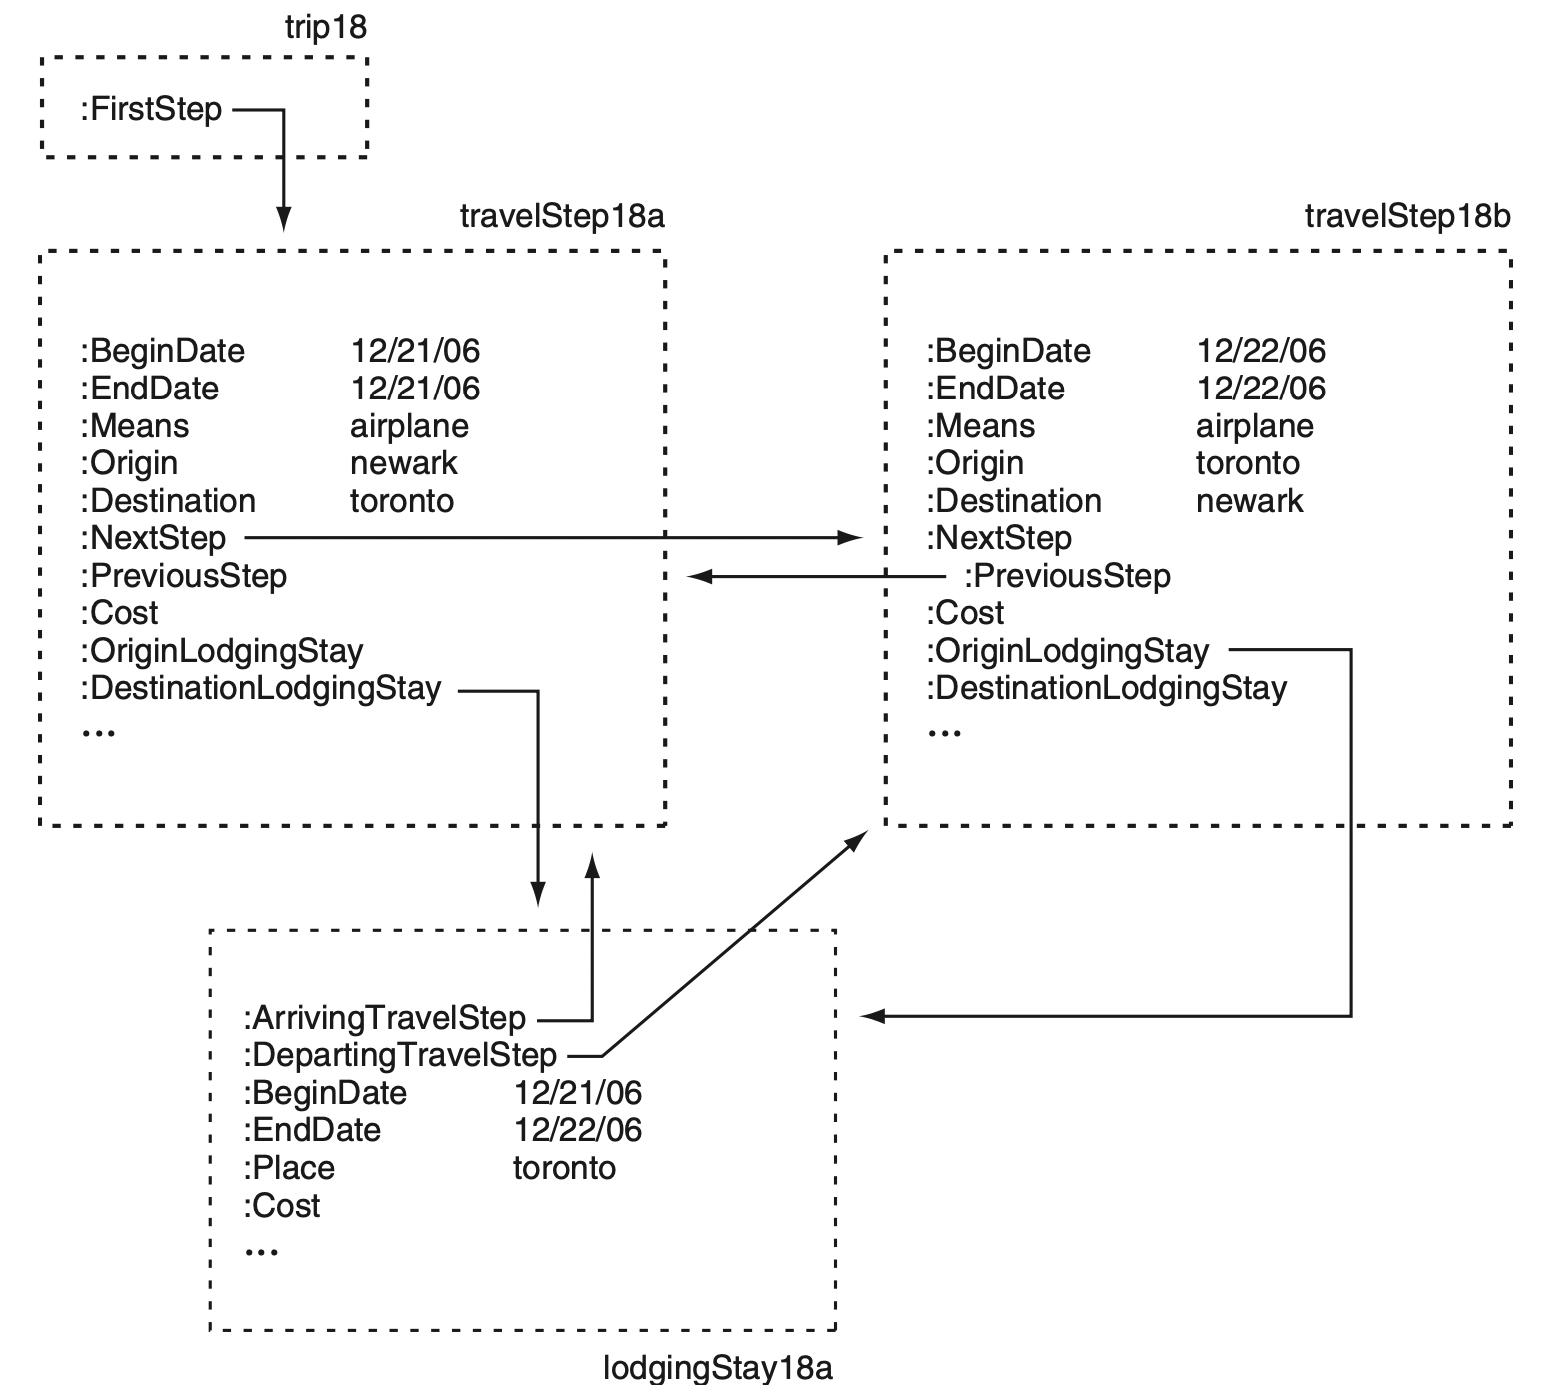
\includegraphics[scale=0.32]{frame.png}
			
		\end{minipage}%
		
	\end{frame}
	
	%------------------------------------------------
	% Representación del conocimiento orientada a objetos 
	\begin{frame}
		
		\frametitle{Representación del conocimiento orientada a objetos }
		
		La representación orientada a objetos desvía el enfoque de la información verdadera hacia las categorías de los objetos y sus propiedades.
		
	\end{frame}
	
	%------------------------------------------------
	% Modelo de representación del conocimiento basado en herencia
	\begin{frame}
		
		\frametitle{Modelo de representación del conocimiento basado en herencia}
		
		\begin{itemize}
			\item La jerarquía de la herencia se define sobre un grafo $\Gamma = <V, E>$ dirigido y acíclico (DAG) con aristas de pesos positivos y negativos. 
			
			\vspace{1\baselineskip}
			\item La herencia es el resultado del razonamiento transitivo sobre un camino del grafo.
			
			\vspace{1\baselineskip}
			\item Un nodo representa una entidad del mundo real.
		\end{itemize}
		
	\end{frame}
	
	%------------------------------------------------
	% Tipos de herencia
	\begin{frame}
		
		\frametitle{Tipos de herencia}
		
		\begin{enumerate}
			
			\only<1>{
				\item[1.] Estricta en árboles
				
				\vspace{1\baselineskip}
				\begin{minipage}{0.43\textwidth} % Primera columna
					
					 \begin{itemize}
					 	\item Un camino produce una conclusión (razonamiento).
					 	
					 	\item Todos los nodos accesibles están implícitos.
					 	
					 	\item Las conclusiones son producidas por un cierre transitivo completo sobre todos los caminos.
					 	
					 \end{itemize}
					
				\end{minipage}
				\hfill  % Espacio entre las columnas
				\begin{minipage}{0.43\textwidth} % Segunda columna
					
					\centering
					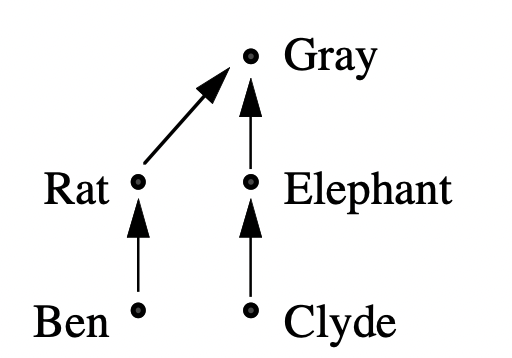
\includegraphics[scale=0.5]{herencia-directa-arbol.png}
					
					\vspace{2\baselineskip}
					La flecha indica un peso positivo.
					
				\end{minipage}
			}
			
			\only<2>{
				\item[2.] Estricta en DAG
				
				\vspace{1\baselineskip}% Primera columna
					
				\begin{itemize}
					\item Puede existir múltiples parientes, o sea, herencia múltiple.
					
					\item Todas las conclusiones a las que se pueden llegar por cualquier camino están respaldadas.
					
				\end{itemize}
				
				\vspace{2\baselineskip}
				\centering
				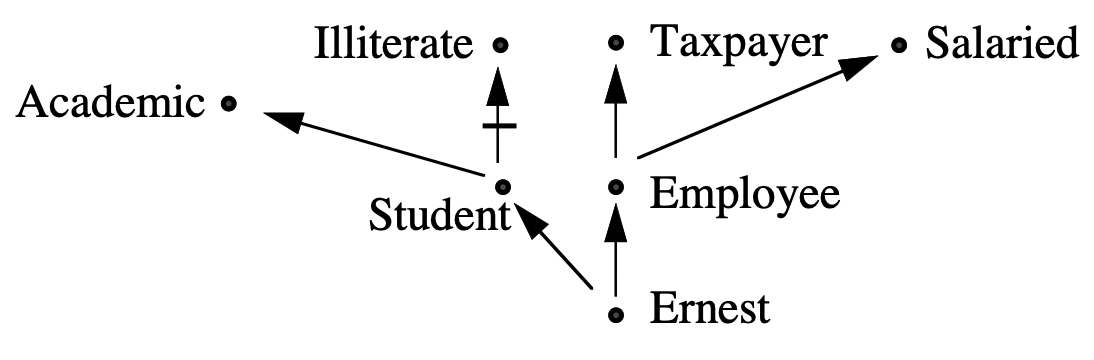
\includegraphics[scale=0.5]{herencia-dag.png}
				
				\vspace{1\baselineskip}
				La flecha cortada indica arista de peso negativo.			
			}
			
			\only<3>{
			
				\item[3.] Cancelable
				
				\vspace{1\baselineskip}
				\begin{minipage}{0.43\textwidth} % Primera columna
					
					\begin{itemize}
						\item Las propiedades heredadas no siempre se mantienen y pueden anularse o sobrescribirse.
						
						\item Las conclusiones están determinadas partiendo del nodo de interés y seleccionando la versión que se desee.
						
						\item Esta representación trae consigo la ambigüedad de las conclusiones.
						
					\end{itemize}
					
				\end{minipage}
				\hfill  % Espacio entre las columnas
				\begin{minipage}{0.43\textwidth} % Segunda columna
					
					\centering
					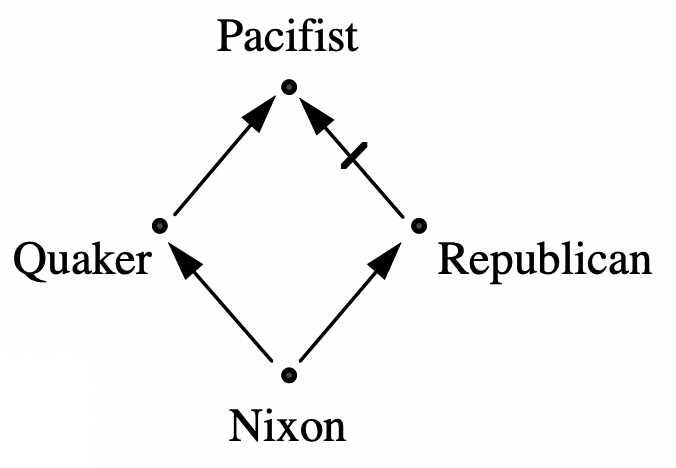
\includegraphics[scale=0.5]{herencia-cancelable.png}
					
					\vspace{2\baselineskip}
					¿Nixon es pacifista?
					
				\end{minipage}
		
			}
			
		\end{enumerate}
		
	\end{frame}
	
	%------------------------------------------------
	% Otras propiedades en los DAG de herencia
	\begin{frame}
		
		\frametitle{Otras propiedades en los DAG de herencia}
		
		\begin{itemize}
			\item El grafo $\Gamma$ es \textbf{$a$-conexo} si $\forall x, a, x \in V(\Gamma)$ existe un camino de aristas con peso positivo entre $a$ y $x$.
			
			\vspace{1\baselineskip}
			\item El grafo $\Gamma$ es \textbf{ambiguo} con respecto a $a \in V(\Gamma)$ si $\exists x \in V(\Gamma)$ tal que existen dos camino distintos entre $a$ y $x$ de modo que un camino solo tiene aristas de peso positivo y el otro camino contiene una arista de peso negativo hacia $x$.
			
			\vspace{1\baselineskip}
			\item Una \textbf{extensión crédula} de $\Gamma$ con respecto al nodo $a \in V(\Gamma)$ es un subgrafo $a$-conexo no ambiguo maximal de $\Gamma$. \\[3mm]
			
			\centering
			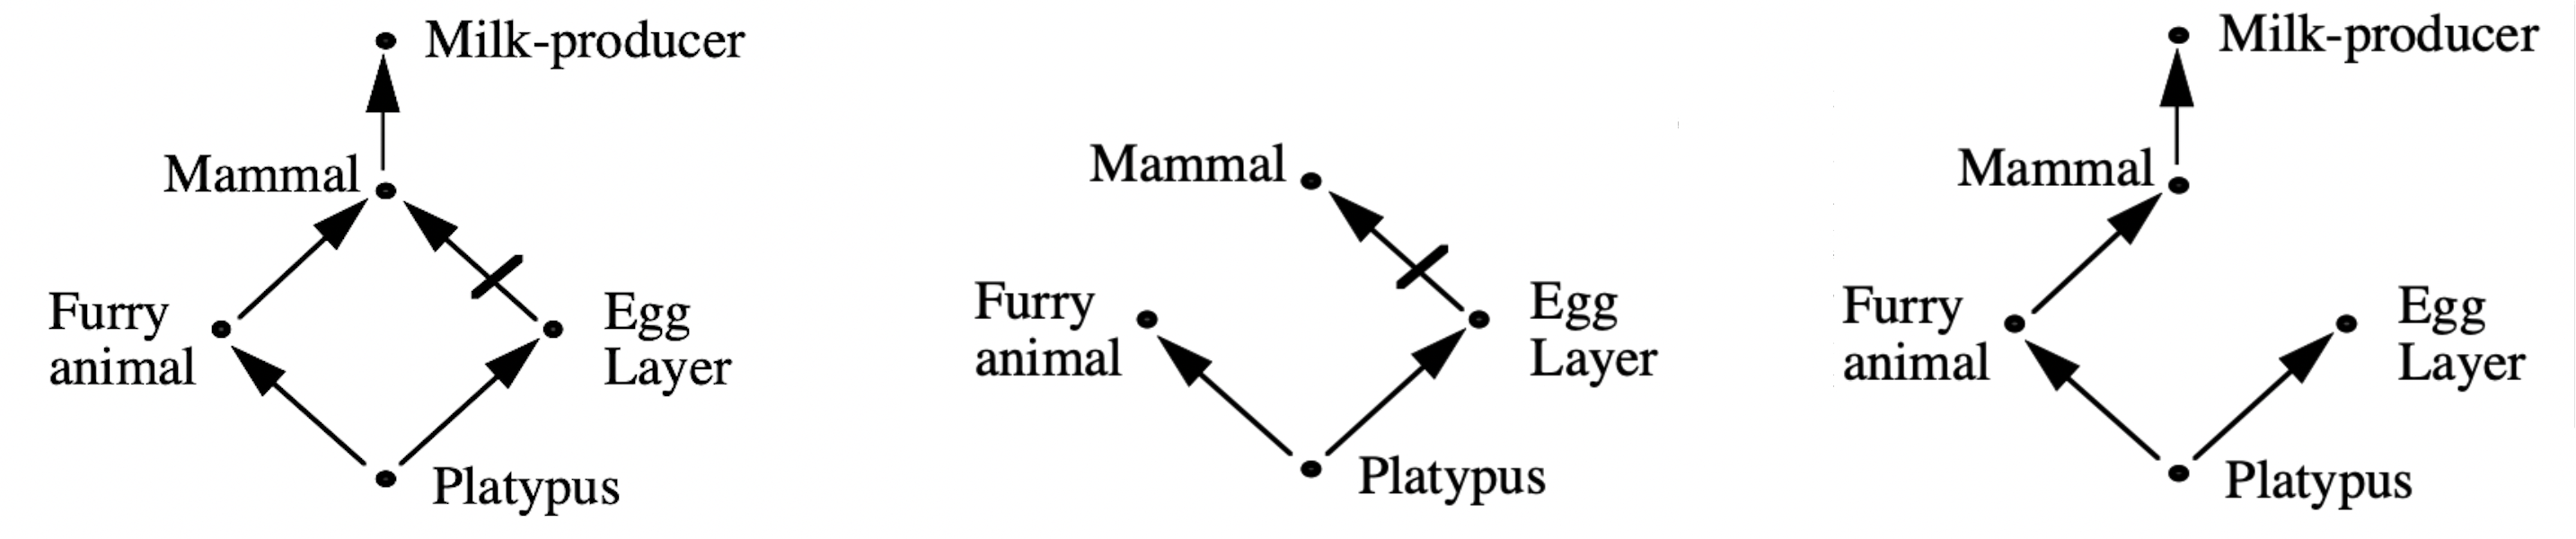
\includegraphics[scale=0.27]{credula.png}
			
		\end{itemize}
		
	\end{frame}
	
	%------------------------------------------------
	% Tipos de razonamientos en la representación basada en herencia
	\begin{frame}
		
		\frametitle{Tipos de razonamientos en la representación basada en herencia}
		
		\begin{itemize}
			
			\item Crédulo \\[1mm]
			Crea todas las conclusiones respaldadas a partir de un extensión.
			
			\vspace{1.5\baselineskip}
			
			\item Escéptico \\[1mm]
			Cree en las conclusiones de cualquier camino que esté respaldado por todas las extensiones preferidas.
			
			\vspace{1.5\baselineskip}
			\item Idealmente escéptico \\[1mm]
			Cree en las conclusiones que están respaldadas por todas las extensiones preferidas. 
			
		\end{itemize}
		
		\pause	
		\centering
		\vspace{3\baselineskip}
		Todo razonamiento se realiza ``hacia arriba''.
		
	\end{frame}
	
	%------------------------------------------------
	% Break
	{
		\setbeamertemplate{background canvas}
		{%
			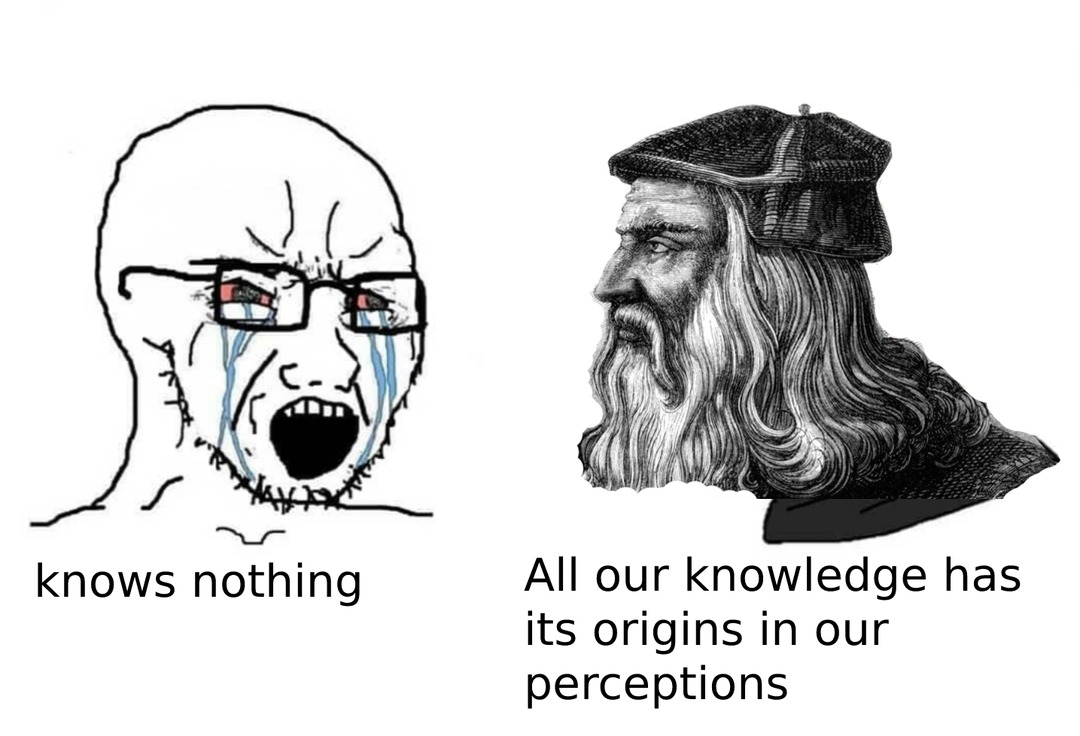
\includegraphics[width=\paperwidth,height=\paperheight]{break-1.jpeg}
		}
		
		\begin{frame}
		\end{frame}
	}
	
	%------------------------------------------------
	% SRI
	\begin{frame}
		
		\frametitle{Sistema de Recuperación de Información (de documentos)}
		
		\centering
		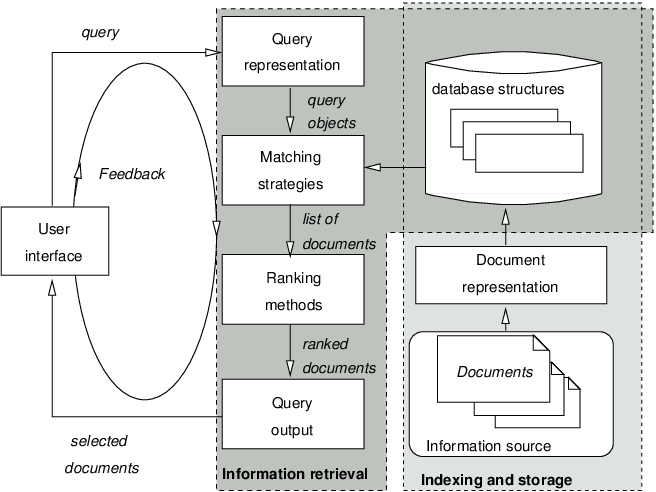
\includegraphics[scale=0.8]{sri.png}
		
		{\scriptsize Tomado de ``Ricarte, Ivan \& Gomide, Fernando. (2004). A Reference Software Model for Intelligent Information Search. 10.1007/978-3-540-45218-8\_14.''}
		
	\end{frame}
	
	%------------------------------------------------
	% Indexación
	\begin{frame}
		
		\frametitle{Obtención de la información almacenada en memoria}
		
		Acceder a la información almacenada en el menor tiempo posible es una tarea de todo sistema computacional que opere con datos en memoria. \\[4mm]
		
		
		\only<1-2>{
			\textcolor{purple}{¿Qué técnica permite acceder y obtener rápido la información almacenada en memoria?}\\[2mm]
		}
		
		\only<2>{
			\textcolor{purple}{¿Qué es la indexación?}
		}
		
		\only<3>{
			\begin{alertblock}{Indexación}
				Identificación de términos o conceptos claves que representan el contenido de cada documento, imagen, sonido u otros datos dentro de un sistema computacional.
			\end{alertblock}
		}
	
	\end{frame}
	
	%------------------------------------------------
	% Importancia de la indexación
	\begin{frame}
		
		\frametitle{Importancia de la indexación}
		
		\begin{itemize}
			\item Mejora la eficiencia de la búsqueda
			%: Permite realizar búsquedas rápidas y precisas en grandes colecciones de documentos.
			
			\vspace{1\baselineskip}
			\item Facilita la recuperación de información relevante 
			% Permite identificar los documentos que mejor se ajustan a las necesidades del usuario.
			
			\vspace{1\baselineskip}
			\item Permite la organización y la categorización de la información
			% Facilita la navegación y el acceso a la información.
		\end{itemize}
		
	\end{frame}
	
	%------------------------------------------------
	% Tipos de indexación
	\begin{frame}
		
		\frametitle{Tipos de indexación}
		
		\begin{itemize}
			\item Manual \\[1mm]
			Realizada por un humano que identifica y selecciona los términos o conceptos claves que representan el contenido de la información.
			
			\vspace{1\baselineskip}
			\item Automática \\[1mm]
			Realizada por un software que utiliza técnicas de procesamiento para identificar, extraer y seleccionar los términos o conceptos clave de la información.
			
		\end{itemize}
		
	\end{frame}
	
	%------------------------------------------------
	% Técnicas de indexación
	\begin{frame}
		
		\frametitle{Técnicas de indexación}
		
		\begin{minipage}[t]{0.43\textwidth} % Primera columna
			
			\begin{itemize}
				
				\item \textcolor<2,3>{gray}{
					Por token (palabra clave) \\[1mm]
					Se basa en la identificación de tokens para representar el contenido de la información.
				}
				
				\vspace{1\baselineskip}
				\item \textcolor<1,3>{gray}{
					Por términos \\[1mm]
					Se basa en la identificación de términos controlados de un vocabulario predefinido que representan el contenido de la información.
				}
				
				\vspace{1\baselineskip}
				\item \textcolor<1,2>{gray}{
					Por conceptos \\[1mm]
					Se basa en la identificación de conceptos que representan el contenido del documento.
				}
				
			\end{itemize}

		\end{minipage}
		\hfill  % Espacio entre las columnas
		\begin{minipage}[t]{0.43\textwidth} % Segunda columna
			
		
		\only<1>{
			\vspace{2\baselineskip}
			Documento: \\``El perro es el mejor amigo del hombre'' \\[2mm]
			Palabras clave: \\perro, amigo, hombre \\[2mm]
			Consulta: \\¿Cuál es el mejor amigo del hombre? \\[2mm]
			Documentos recuperados: \\``El perro es el mejor amigo del hombre.''
		}
		
		\only<2>{
			\vspace{.7\baselineskip}
			Documento: \\``El perro es el mejor amigo del hombre.''\\[2mm]
			Términos: \\perro (animal doméstico, canino), amigo (compañero, confidente), hombre (ser humano, varón)\\[2mm]
			Consulta: \\¿Cuál es la relación entre el perro y el hombre?\\[2mm]
			Documentos recuperados: \\``El perro es el mejor amigo del hombre.'' \\``El perro y el hombre: una historia de amistad.''
		}
		
		\only<3>{
			\vspace{1.3\baselineskip}
			Documento: \\``El perro es el mejor amigo del hombre.''\\[2mm]
			Conceptos: \\perro (mascota, lealtad), amigo (compañía, apoyo), hombre (familia, sociedad)\\[2mm]
			Consulta: \\¿Cuál es el papel del perro en la sociedad?\\[2mm]
			Documentos recuperados: \\``El perro es el mejor amigo del hombre.''\\``El perro: un miembro de la familia."
		}
			
		\end{minipage}
		
	\end{frame}
	
	%------------------------------------------------
	% 1 - Algoritmos para almacenar la información indexada
	\begin{frame}
		
		\frametitle{Algoritmos para almacenar la información indexada}
		
		\begin{itemize}
			\item Indexación basada en clasificación bloqueada \\[2mm]
			% El método de indexación basada en ordenación por bloques (BSBI) es un algoritmo eficiente para la construcción de índices invertidos en grandes colecciones de documentos
			
			\item Indexación en memoria de un solo paso \\[2mm]
			% El método de indexación en memoria de un solo paso (SPIMI) es un algoritmo eficiente para la construcción de índices invertidos en memoria principal.	
			
			\item Indexación distribuida \\[2mm]
			% La indexación distribuida es un método para construir un índice invertido para una gran colección de documentos utilizando múltiples computadoras.
			
			\item Indexación dinámica
			% Es un método de indexación que actualiza el índice invertido de forma incremental a medida que se añaden nuevos documentos a la colección. 
			
		\end{itemize}
		
	\end{frame}
	
	%------------------------------------------------
	
	%------------------------------------------------
	% 1 - Algoritmos para almacenar la información indexada
	\begin{frame}
		
		\frametitle{Algoritmos para almacenar la información indexada}
		
		\begin{itemize}
			\item Indexación basada en clasificación bloqueada (Blocked sort-based indexing, BSBI)
			% El método de indexación basada en ordenación por bloques (BSBI) es un algoritmo eficiente para la construcción de índices invertidos en grandes colecciones de documentos
			
			\vspace{1\baselineskip}
			
			\begin{itemize}
				
				\pause
				\item Algoritmo (pasos) \\[1mm]
				\begin{enumerate}
					\item La colección de datos se divide en bloques de tamaño fijo.
					\item Cada bloque se indexa de forma independiente, utilizando un algoritmo de ordenación para crear un índice invertido para los términos del bloque.
					\item Los índices invertidos de cada bloque se fusionan en un único índice invertido para la colección completa.
				\end{enumerate}
				
				\pause 
				\begin{minipage}[t]{0.43\textwidth} % Primera columna
					
					\item Ventajas:
					\begin{itemize}
						\item Eficiente 
						\item Escalable
						\item Simple
					\end{itemize}
					
				\end{minipage}
				\hfill  % Espacio entre las columnas
				\begin{minipage}[t]{0.43\textwidth} % Segunda columna
					
					\item Desventajas:
					\begin{itemize}
						\item Requiere memoria 
						\item No es incremental
					\end{itemize}
					
				\end{minipage}
				
			\end{itemize}
					
		\end{itemize}
		
	\end{frame}
	
	%------------------------------------------------
	% 2 - Algoritmos para almacenar la información indexada
	\begin{frame}
		
		\frametitle{Algoritmos para almacenar la información indexada}
		
		\begin{itemize}
			\item Indexación en memoria de un solo paso (Single-pass in-memory indexing, SPIMI)
			% El método de indexación en memoria de un solo paso (SPIMI) es un algoritmo eficiente para la construcción de índices invertidos en memoria principal.	
						
			\vspace{1\baselineskip}
				
			\begin{itemize}
				
				\pause
				\item Algoritmo (pasos)
				\begin{enumerate}
					\item Los datos se leen de uno en uno.
					\item Cada dato pasa por un proceso de extracción de términos para identificar aquellos individuales.
					\item Se crea una lista de publicaciones para cada término que contiene los identificadores de los datos en los que aparece el término.
					\item La lista de publicaciones se escribe en disco una vez que se procesa un bloque de documentos.
				\end{enumerate}
				
				\pause 
				
				\begin{minipage}[t]{0.43\textwidth} % Primera columna
					
					\item Ventajas:
					\begin{itemize}
						\item Eficiente 
						\item Escalable
						\item Simple
					\end{itemize}
					
				\end{minipage}
				\hfill  % Espacio entre las columnas
				\begin{minipage}[t]{0.43\textwidth} % Segunda columna
					
					\item Desventajas:
					\begin{itemize}
						\item Requiere memoria 
						\item No es incremental
					\end{itemize}
					
				\end{minipage}
				
			\end{itemize}

		\end{itemize}
				
	\end{frame}
	
	%------------------------------------------------
	% 3 - Algoritmos para almacenar la información indexada
	\begin{frame}
		
		\frametitle{Algoritmos para almacenar la información indexada}
		
		\begin{itemize}
			\item Indexación distribuida 
			% La indexación distribuida es un método para construir un índice invertido para una gran colección de documentos utilizando múltiples computadoras.
			% Aprovecha las bpndades de MapReduce.
			
			\vspace{1\baselineskip}	
			
			\begin{itemize}
				
				\pause
				\item Algoritmo (pasos)
				\begin{enumerate}
					\item La colección de datos se divide en subcolecciones más pequeñas.
					\item Cada subcolección se indexa de forma paralela en una computadora diferente.
					\item Los índices invertidos de cada subcolección se fusionan en un único índice invertido para la colección completa.
				\end{enumerate}
				
				\pause 
				
				\begin{minipage}[t]{0.43\textwidth} % Primera columna
					
					\item Ventajas:
					\begin{itemize}
						\item Eficiente
						\item Escalable
						\item Disponibilidad 
						% La indexación distribuida puede mejorar la disponibilidad del sistema, ya que la falla de una computadora no afecta a la indexación de otras subcolecciones.
					\end{itemize}
					
				\end{minipage}
				\hfill  % Espacio entre las columnas
				\begin{minipage}[t]{0.43\textwidth} % Segunda columna
					
					\item Desventajas:
					\begin{itemize}
						\item Complejo
						% La indexación distribuida es un algoritmo más complejo de implementar que la indexación secuencial.
						\item Costoso 
						% La indexación distribuida puede requerir más recursos informáticos que la indexación secuencial.
					\end{itemize}
					
				\end{minipage}
				
			\end{itemize}
			
		\end{itemize}
		
	\end{frame}
	
	%------------------------------------------------
	% 4 - Algoritmos para almacenar la información indexada
	\begin{frame}
		
		\frametitle{Algoritmos para almacenar la información indexada}
		
		\begin{itemize}
			\item Indexación dinámica
			% Es un método de indexación que actualiza el índice invertido de forma incremental a medida que se añaden nuevos documentos a la colección. 
			
			\vspace{1\baselineskip}	

		
			\begin{itemize}
				
				\pause
				\item Algoritmo (pasos)
				\begin{enumerate}
					\item Se crea un índice invertido inicial para la colección de datos existente.
					\item Cuando se añade un nuevo dato a la colección, se actualiza el índice invertido para incluir los términos del nuevo documento.
					\item Cuando se elimina un dato de la colección, se elimina del índice invertido.
				\end{enumerate}	
		
				\pause 
				\begin{minipage}[t]{0.43\textwidth} % Primera columna
					
					\item Ventajas:
					\begin{itemize}
						\item Eficiente
						\item Escalable
						\item Flexible				
					\end{itemize}
					
				\end{minipage}
				\hfill  % Espacio entre las columnas
				\begin{minipage}[t]{0.43\textwidth} % Segunda columna
					
					\item Desventajas:
					\begin{itemize}
						\item Complejo 
							% La indexación dinámica es un algoritmo más complejo que la indexación estática.
						\item Costoso de mantener 
							% La indexación dinámica puede tener un impacto en el rendimiento del sistema, especialmente en colecciones de datos que se actualizan con mucha frecuencia.
					\end{itemize}
					
				\end{minipage}
	
			\end{itemize}
			
		\end{itemize}		
		
	\end{frame}
	
	%------------------------------------------------
	% Break
	{
		\setbeamertemplate{background canvas}
		{%
			
\includegraphics[width=\paperwidth,height=\paperheight]{break-2.jpg}
		}
		
		\begin{frame}
		\end{frame}
	}
	
	%------------------------------------------------
	% Conclusiones
	\begin{frame}
		
		\frametitle{Conclusiones}
		
		\begin{itemize}
			
			\item La computación ofrece herramientas para la representación y el manejo del conocimiento, así como para el razonamiento automático. \\[2mm]
			
			\item Cada tipo de representación del conocimiento tiene sus ventajas y desventajas, y la elección de la representación adecuada depende del problema a resolver. \\[2mm]
			
			\item La indexación es un proceso fundamental para la recuperación de información.
			
		\end{itemize}
		
	\end{frame}
	
	%------------------------------------------------
	% Bibliografía
	\begin{frame}
		
		\frametitle{Bibliografía}
		
		\begin{itemize}
			
			\item Brachman, Ron J.; Levesque, Hector J. (2004) Knowledge Representation and Reasoning. ELSEVIER. Capítulos 7, 8, 10.
			
			\item Manning, Christopher D.; Raghavan, Prabhakar; Schütze, Hinrich (2007). An Introduction to Information Retrieval. Capítulo 4.
			
		\end{itemize}
		
	\end{frame}
	
	%------------------------------------------------
	% Fin
	\begin{frame}
		\titlepage
	\end{frame}
	
	
	
\end{document} 